\textbf{a,} Ta đặt $r = \sqrt{x^2 + y^2}$ là toạ độ khoảng cách trong mặt phẳng $Oxy$. Từ phương trình ném xiên, tuân theo định luật Newton II, ta có phương trình chuyển động của mảnh đạn:
\begin{align}
    z &= -\frac{1}{2} g t^2 + v_0 \sin \theta t + H, \label{1}\\
    r&= v_0 \cos \theta t. \label{2}
\end{align}

Thay (\ref{1}) vào (\ref{2}) ta thu được phương trình quỹ đạo của mảnh đạn là
\begin{align}
    z = H- \frac{g}{2 v_0^2 \cos^2 \theta} r^2 + r \tan \theta. \label{3}
\end{align}

Ta có thể viết (\ref{3}) thành phương trình tam thức bậc hai với biến $\tan \theta$ như sau
\begin{align}
    - \frac{g r^2}{2 v_0^2} \tan^2 \theta + r \tan \theta - \left( \frac{g r^2}{2 v_0} + z -H \right) = 0.\label{4}
\end{align}

\begin{itemize}\itemsep0em
\item Bên ngoài ranh giới, tức vùng an toàn, thì phương trình (\ref{4}) vô nghiệm.

\item Bên trong ranh giới, tức vùng nguy hiểm, thì phương trình (\ref{4}) có hai nghiệm phân biệt.

\item Tại ranh giới thì phương trình (\ref{4}) là nghiệm kép, tức là $\Delta = 0$.
\end{itemize}



Từ nhận xét trên ta có phương trình
\begin{align}
    \Delta &= r^2 - 4 \frac{gr^2}{2 v_0^2} \left( \frac{gr^2}{2v_0^2} + z-H \right) = 0,\\
    \Rightarrow z &= H + \frac{v_0^2}{2g} - \frac{gr^2}{2 v_0^2} = H + \frac{v_0^2}{2g} - \frac{g}{2 v_0^2} (x^2 + y^2).\label{10}
\end{align}

Hình bên dưới là mô phỏng đường ranh giới an toàn của bom nổ.

\begin{center}
    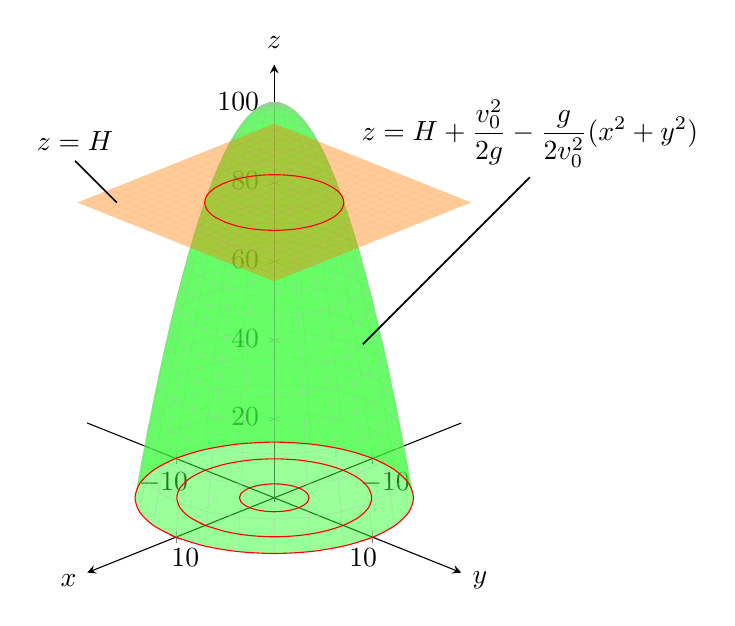
\begin{tikzpicture}
\begin{axis}[
xlabel=$x$, ylabel=$y$, zlabel=$z$, 
xmin=-19, xmax=19,
ymin=-19, ymax=19,
zmin=-1, zmax=110,
x={(-0.125cm,-0.05cm)}, y={(0.125cm,-0.05cm)}, z={(0cm,0.05cm)},
axis lines=middle,
every axis x label/.style={  at={(ticklabel* cs:1.05)},  },
every axis y label/.style={  at={(ticklabel* cs:1.05)},  },
every axis z label/.style={  at={(ticklabel* cs:1.05)},  },
]
% Paraboloid
\addplot3[surf,
shader=flat, draw=lightgray, fill=green!80, ultra thin, 
left color=green, right color=green, middle color=green!25, 
opacity=0.5, fill opacity=0.5,
data cs=polar, domain=0:360, 
y domain=0:10,
restrict z to domain=0:101, 
](x, y, 100-y^2);

% Plane 
\addplot3[surf, shader=faceted,
color=orange, 
opacity=0.01, fill opacity=0.4, 
domain=-10:10, 
](x,y,75);

% Circle at plane
\addplot3[red, smooth, 
domain=0:360, variable=\t
]({5*cos(\t)},{5*sin(\t)},{75});

% Circles at xy-plane
\pgfplotsinvokeforeach{10, 7, 2.5}{%%
\pgfmathsetmacro\Radius{#1}
\addplot3[red, smooth, 
%no markers,
%samples=55,% samples y=0, 
domain=0:360, variable=\t
]({\Radius*cos(\t)},{\Radius*sin(\t)},{0});
}%%

% Annotations 1/2
\coordinate[label=](A) at ({7*cos(135)},{7*sin(135)},{0});
\coordinate[label=](B) at (8, -8, 75);
\coordinate[label=](C) at (-4, 5, 40);
\coordinate[label=](D) at({5*cos(300)},{5*sin(300)},{75});
\end{axis}



\draw[semithick] (B) -- +(135:0.75) node[above, align=left]{
$z=H$};

\draw[semithick] (C) -- +(45:3) node[above]{$\displaystyle z=H + \frac{v_0^2}{2g} - \frac{g}{2v_0^2} (x^2 + y^2)$};


\end{tikzpicture}  
\end{center}

\textbf{b,} Bán kính của vùng đạn là 
\begin{align}
    R = r(z=0) = \frac{v_0}{g} \sqrt{2gH + v_0^2}.\label{11}
\end{align}


\textbf{c,} Gọi góc phương vị (tạo bởi đường xiên và phương $z$) là $\displaystyle \alpha = \frac{\pi}{2} - \theta$.

Tầm xa của mảnh đặn bắn với góc nhìn $\theta$ là
\begin{align}
    r = \frac{v_0^2}{g} \sin 2 \theta = \frac{v_0^2}{g} \sin 2 \alpha. \label{5}
\end{align}

Vi phân khối lượng đạn $dm$ được bắn ra từ góc $\alpha \rightarrow \alpha + d\alpha$ (hệ toạ độ cầu) là 
\begin{align}
    dm = M \frac{2 \pi \sin \alpha d\alpha}{\displaystyle 2 \pi \int_0^{\alpha_0} \sin \alpha d\alpha} = \frac{M \sin \alpha d\alpha}{1 - \cos \alpha_0} \approx \frac{2M}{\alpha_0^2} \sin \alpha d\alpha. \label{12}
\end{align}

Phân bố khối lượng đạn trên sàn nhà thoả mãn
\begin{align}
    \rho (r) 2 \pi r dr &= dm = \frac{2M}{\alpha_0^2} \sin \alpha d\alpha\\
 \Rightarrow   \rho(r) &= \frac{2M \sin \alpha}{\pi \alpha_0^2} \frac{d\alpha}{d(r^2)}.\label{7}
\end{align}

Bình phương rồi đạo hàm (\ref{5}) ta thu được 
\begin{align}
    \frac{d(r^2)}{d\alpha} = \frac{2v_0^2}{g^2} \sin 4 \alpha \approx \frac{8v_0^2}{g} \alpha \left(1 - \frac{8}{3} \alpha^2 \right).\label{6}
\end{align}

Lắp (\ref{6}) vào (\ref{7}) ta thu được 
\begin{align}
    \rho(r) &= \frac{M g^2}{4 \pi v_0^4 \alpha_0^2} \frac{1 - \dfrac{1}{6}\alpha^2}{1 - \dfrac{8}{3}\alpha^2}\\
    &\approx  \frac{M g^2}{4 \pi v_0^4 \alpha_0^2} \left( 1 - \frac{1}{6}\alpha^2\right) \left( 1 + \frac{8}{3}\alpha^2\right)\\
    & \approx  \frac{M g^2}{4 \pi v_0^4 \alpha_0^2} \left( 1 + \frac{5}{2} \alpha^2 \right)\\
    & =  \frac{M g^2}{4 \pi v_0^4 \alpha_0^2} \left( 1 + \frac{5g^2}{8 v_0^4} r^2 \right).
\end{align}

Vậy ta có các hệ số cần tìm là $\displaystyle \rho_0 =  \frac{M g^2}{4 \pi v_0^4 \alpha_0^2}$ và $\displaystyle \beta = \frac{5g^2}{8 v_0^4}$.

\vspace{2mm}

 \textbf{Biểu điểm} 
\begin{center}
\begin{tabular}{|>{\centering\arraybackslash}m{1cm}|>{\raggedright\arraybackslash}m{14cm}| >{\centering\arraybackslash}m{1cm}|}
    \hline
    \textbf{Phần} & \textbf{Nội dung} & \textbf{Điểm} \\
    \hline
    \textbf{a} & Viết được tam thức bặc hai với $\tan \theta$ (\ref{4}) & 0.50\\   
    \cline{2-3}
    &  Việt được phương trình đường ranh giới (\ref{10}) & 1.00\\
    \cline{2-3}
    & Vẽ phác đồ thị, đúng dạng paraboloid, có chú thích & 0.50\\
    \hline
    \textbf{b} & Biểu diễn đúng $R$ (\ref{11}) & 0.50 \\
    \hline
    \textbf{c} & Biểu diễn được vi phân $dm$ (\ref{12}) & 0.50\\
    \cline{2-3}
    & Biển diễn được $\rho(r)$ theo $d\alpha$ và $dr$ (\ref{7}) & 0.50\\
    \cline{2-3}
    & Tìm được các hệ số $\rho_0$ và $\beta$ & 0.50\\
    \hline
\end{tabular}
\end{center}

\noindent \textbf{Mở rộng vấn đề:}

Bài toán này được trích từ bài 3 đề 1 trong đề Olympic đồng bằng sông Châu Giang 2016 (Pan Pear River Delta Physics Olympiad). Đây không phải một bài toán khó, song hầu hết các học sinh vật lý giải sai do sự thiếu chặt chẽ trong các tính toàn về khai triển nhỏ (Rất nhiều người ra hệ số của $\beta$ là 1/2 hoặc 1/24 do bỏ mất các hạng tử nhỏ đồng bậc). 